%%%%%%%%%%%%%%%%%%%%%%%%%%%%%%%%%%%%%%%%%
% Journal Article
% LaTeX Template
% Version 1.3 (9/9/13)
%
% This template has been downloaded from:
% http://www.LaTeXTemplates.com
%
% Original author:
% Frits Wenneker (http://www.howtotex.com)
%
% License:
% CC BY-NC-SA 3.0 (http://creativecommons.org/licenses/by-nc-sa/3.0/)
%
%%%%%%%%%%%%%%%%%%%%%%%%%%%%%%%%%%%%%%%%%

%----------------------------------------------------------------------------------------
%	PACKAGES AND OTHER DOCUMENT CONFIGURATIONS
%----------------------------------------------------------------------------------------

\documentclass[twoside]{article}

\usepackage{lipsum} % Package to generate dummy text throughout this template

\usepackage[sc]{mathpazo} % Use the Palatino font
\usepackage[T1]{fontenc} % Use 8-bit encoding that has 256 glyphs
\linespread{1.05} % Line spacing - Palatino needs more space between lines
\usepackage{microtype} % Slightly tweak font spacing for aesthetics
\usepackage{paralist}
\usepackage[margin={1.5cm,1.5cm},top=32mm,columnsep=20pt]{geometry} % Document margins
\usepackage{multicol} % Used for the two-column layout of the document
\usepackage[hang, small,labelfont=bf,up,textfont=it,up]{caption} % Custom captions under/above floats in tables or figures
\usepackage{booktabs} % Horizontal rules in tables
\usepackage{graphicx,float}
\usepackage{float} % Required for tables and figures in the multi-column environment - they need to be placed in specific locations with the [H] (e.g. \begin{table}[H])
\usepackage{hyperref} % For hyperlinks in the PDF
\usepackage{amsmath,amsfonts,amsthm}
\usepackage{lettrine} % The lettrine is the first enlarged letter at the beginning of the text
\usepackage{paralist} % Used for the compactitem environment which makes bullet points with less space between them

\usepackage{abstract} % Allows abstract customization
\renewcommand{\abstractnamefont}{\normalfont\bfseries} % Set the "Abstract" text to bold
\renewcommand{\abstracttextfont}{\normalfont\small\itshape} % Set the abstract itself to small italic text

\usepackage{algorithm}
\usepackage[noend]{algpseudocode}
\makeatletter
\def\BState{\State\hskip-\ALG@thistlm}
\makeatother

\usepackage{titlesec} % Allows customization of titles
\renewcommand\thesection{\arabic{section}} % Roman numerals for the sections
\renewcommand\thesubsection{\arabic{subsection}} % Roman numerals for subsections
\titleformat{\section}[block]{\Large\scshape\centering}{\thesection.}{1em}{} % Change the look of the section titles
\titleformat{\subsection}[block]{\large}{\thesection.\thesubsection.}{1em}{} % Change the look of the section titles

\usepackage{fancyhdr} % Headers and footers
\pagestyle{fancy} % All pages have headers and footers
\fancyhead{} % Blank out the default header
\fancyfoot{} % Blank out the default footer
\fancyhead[C]{Userless Classificaton for the Yelp Dataset Challenge} % Custom header text
\fancyfoot[RO,LE]{\thepage} % Custom footer text

%----------------------------------------------------------------------------------------
%	TITLE SECTION
%----------------------------------------------------------------------------------------

\title{\vspace{-15mm}\fontsize{24pt}{10pt}\selectfont\textbf{Userless Classificaton for the Yelp Dataset Challenge}} % Article title

\author{
\large
\textsc{Nicolas Drizard \& Virgile Audi}\\[2mm] % Your name
\normalsize Final Project for CS281, Harvard University \\ % Your institution
\normalsize {nicolas.drizard@g.harvard.edu \quad vaudi@g.harvard.edu} % Your email address
\vspace{-5mm}
}
\date{}

%----------------------------------------------------------------------------------------

\begin{document}

\maketitle % Insert title

\thispagestyle{fancy} % All pages have headers and footers

%----------------------------------------------------------------------------------------
%	ABSTRACT
%----------------------------------------------------------------------------------------

\begin{abstract}

\noindent

We planned on building latent features from the text reviews which would depict the cat- egories of the business. To put it in a nutshell, we would like to build from the text reviews of an entry a vector representation which carries local geometry information. Once we built the document-term matrix containing the words count of the reviews for each business (the reviews are aggregated over each restaurant), we could simply use a matrix factorisation on the counts . To be able to interpret the latent features as topics, we could use a Non-negative matrix factorization (the possible negative features in the SVD cannot stand for cluster as- signement). A finer result can be reached with the use of a generative probabilistic model, that’s why we chosed the latent dirichlet allocation. The LDA uses a Dirichlet prior on the words distribution over the topics and on the topics distribution over the document which will gives them more freedom than the deterministic approach of the NMF.

\end{abstract}

%----------------------------------------------------------------------------------------
%	ARTICLE CONTENTS
%----------------------------------------------------------------------------------------

\begin{multicols}{2} % Two-column layout throughout the main article text

\section{Introduction}

\lettrine[nindent=0em,lines=1]{T}he classification system in Yelp is manual. When the owner of a business creates a page for his restaurant or bar, he is asked to enter a certain number of attributes or "tags". Yelp users can then alter or even add some new tags based on their experiences. As part of the Yelp Data Set Challenge Round 6, we decided to tackle the issue of classification with ultimate objective to be able to create an automathised method to classify venues, based on the information contained on the business' webage and most importantly the written reviews from Yelpers. This project can be divided in two parts, the first on Feature Extraction and the second on classification and clustering. In more details, we applied various dimensionality reduction methods such as Latent Dirichlet Allocation (LDA) or Non-negative Matrix Factorisation (NMF) to map the reviews into a geometrical space. We then decided to compare both supervised approaches such as Multinomial Regression and unsupervised approaches, for instance the Walktrap algorithm, to the problem of classification on the Yelp dataset.
%------------------------------------------------

\section{Data}

Yelp provides data on all kinds of venues such as dentists or bars in 5 cities in the United-States and Europe. The data can be summarised as follows:

\begin{compactitem}
	\item 1.6 million reviews
	\item 61 000 businesses		
	\item 481 000 attributes 
	\item aggregated check-in measurements over time
\end{compactitem}

\noindent For simplicity, we chose to focus on restaurants and bars in the city of Las Vegas, Nevada. We reduced the data to a dataset of 3822 businesses, about 20 thousands reviews and 250 other features such as hours, parking availabity, take-out, ambience. If the numerical data we received from Yelp was mostly cleaned, it was not the case of the text data. Cleaning the reviews represented a significant part of this final project. We present some of the steps we followed in the process:\\

\begin{compactitem}
	\item We aggregated all the reviews about a particular business into a "super" review, in order to get a general sense of what the restaurant was about,
	\item We applied spelling corrections, removed common stopwords and generic words such as "table" or "restaurants",
	\item We attempted at only selecting common words and not adjectives in order to focus on what the venues were about and not the users' opinions,
	\item We transformed the corpus of "super reviews" into a document-term matrix that we could exploit.
\end{compactitem}

%------------------------------------------------

\section{Feature Extraction}

\subsection{Approach}

To extract content from the reviews, we applied 2  methods from Topic Modeling to reduce the document term matrix into meaningful information. We first looked at LDA, using both a Gibbs sampler and Online Variational Inference (OVI) algorithm. Note that we used the Gibbs sampler as a way to benchmark our coded OVI. The motivation behind OVI is twofold. First, it appeared more appropriate to the data we were working with, indeed new reviews can always be added to the corpus in continuous flow. Second, it showed some extremely significant time improvement over the Gibbs sampler version in Python (cf figure 1). We also wanted to compare the performance of LDA with a non-probabilistic approach which is NMF. 
  
\subsection{Latent Dirichlet Allocation}

The LDA is a three-level hierarchical Bayesian model. The basic idea that documents are represented as random mixtures over latent topics and each topic is characterized by a distribution over words.\cite{LDA}\\

\noindent The generative process for a document \textbf{w} in a corpus D is the following:
\\
\begin{compactenum}
	\item Choose the topics representation:\newline $\phi \sim$ Dir($\beta$)
	\item Choose the number of words:\newline $ N \sim $ Poisson($ \xi $)
	\item Choose the distribution of topics:\newline $\theta_w \sim$ Dir($\alpha_w$)
	\item For each of the N words:
	\begin{compactenum}
		\item Choose a topic assignement:\newline $z_{n,w} \sim \text{Multinomial}(\theta_w)$
		\item Choose a word: \newline$w_n \sim \text{ Multinomial}(\phi_{z_{n,w}})$
	\end{compactenum}
\end{compactenum}

\begin{figure}[H]
\centering
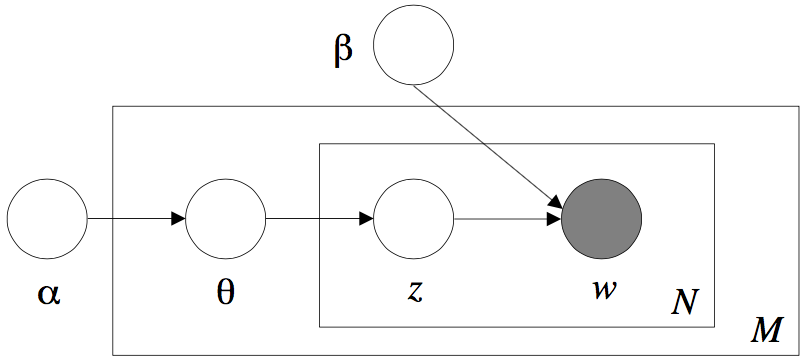
\includegraphics[width=0.8\linewidth]{LDA.png}
\caption{Graphical Model Representation of LDA}
\end{figure}

\subsection{Parameter Estimation and algorithm:}

The main issue relies in computing the posterior distribution of the hidden variables given a document:\\

\begin{align*}
p(\theta, \mathbf{z} |\mathbf{w}, \alpha, \beta) = \frac{p(\theta, \mathbf{z}, \mathbf{w} | \alpha, \beta)}{p(\mathbf{w} | \alpha, \beta)}
\end{align*}

\noindent This distribution is intractable. As mentioned above, we used two  methods to infer it: through a Gibbs sampler or variational inference. In the first case, we are estimating the hyper parameters $\theta$ and $\phi$ with samples on the different variables. Alternatively, we chose the online variational inference method which finds the variational parameters that optimize a lower bound on the loglikelihood. The setup \cite{OLLD} of the Variational Inference is as follows. We first approximate the true posterior by a simpler and factorised distribution:
$$q(\boldsymbol{z},\boldsymbol{\theta},\boldsymbol{\beta}) = q(\boldsymbol{z})q(\boldsymbol{\theta})q(\boldsymbol{\beta}) $$ 

\noindent where:
$$ q(z_{di} = k) = \phi_{d_{w_{di}k}} \quad q(\theta_d) = \text{Dir}(\theta_d,\gamma_d) \quad q(\beta_k) = \text{Dir}(\beta_k,\lambda_k) $$

\noindent The $\boldsymbol{\gamma}$ parameter rule the topic assignments for each document and the $\boldsymbol{\lambda}$, the topics themselves. We then minimise the KL divergence between the distribution $q$ and the true posterior $p$ like for the usual variational inference. What differs in online variational inference is that we sample a batch of document at each step and perform the E-step as if this batch constituted the entire corpus. We present the algorithm below:

\begin{algorithm}[H]
\caption{Batched Online Variational Inference}\label{euclid}
\begin{algorithmic}[1]
\State Define $\rho_t \equiv (\tau_0 + t)^{-\kappa}$
\State Initalise $\boldsymbol{\lambda}$ randomly
\State Sample a batch $\mathcal{S}$ of documents of size S
\For {$d$ in $\mathcal{S}$}
\While {$\gamma_(d)$ hasn't converged}
\State Set $\phi^{(d)}_{twk} \propto \exp\{\mathbb{E}_q\log\theta_{tk} + \mathbb{E}_q\log\beta_{kw}\}$
\State Set $\gamma^{(d)}_{tk} = \alpha + \sum_{w} \phi^{(d)}_{twk}n_{tw}$
\EndWhile
\State Compute $\tilde{\lambda}_{kw} = \eta +\frac{D}{S}n_{tw}\phi^{(d)}_{twk}$
\EndFor
\State $\boldsymbol{\lambda} = (1-\rho_t)\boldsymbol{\lambda}+\rho_t\boldsymbol{\tilde{\lambda}}$
\State $t = t+1$
\State \textbf{goto} 3 and repeat until all documents are observed.
\end{algorithmic}
\end{algorithm}

\noindent where $\kappa \in (0.5,1]$ rules how fast we forget old values of $\tilde{\lambda}$ and $\tau_{0}$ how much weight one wants to put on the first iterations. 

\subsection{Evaluation Method}

We need a measure to evaluate the performance of our model and to tune the hyperparameters. We use perplexity on held-out data as a measure of our model fit. Perplexity is defined as the geometric mean of the log likelihood of the words in the held-out set of docuements given the trained model. In our case, for each document we held out 20\% of the words which constitue the test set.

\begin{align*}
	perplexity(D_{test}) & = \frac{\sum\limits_{d \in D_{test}} \log p(words)}{\sum\limits_{d \in D_{test}|d|}}\\
	perplexity(D_{test}) & = \frac{\sum\limits_{d \in D_{test}} \sum\limits_{w \in d} \log \left( \sum_{t \in topics} p(w|t)p(t|d) \right)}{\sum\limits_{d \in D_{test}|d|}}
\end{align*}

\noindent We used this measure to optimize the number of topics K and the hyper parameters of the optimization. We also used the perplexity to benchmark our algorithm with the Gibbs sampler in the LDA 1.0.3 package in Python:

$$\text{perp}_{OVI} = XX \quad \text{and} \quad \text{perp}_{GS} = XX$$

\subsection{Results}
Another way to assess the performance of our LDA was to inspect the topics outputted by the algorithm. We present some of the most significant topics:\\

\begin{figure}[H]
\centering
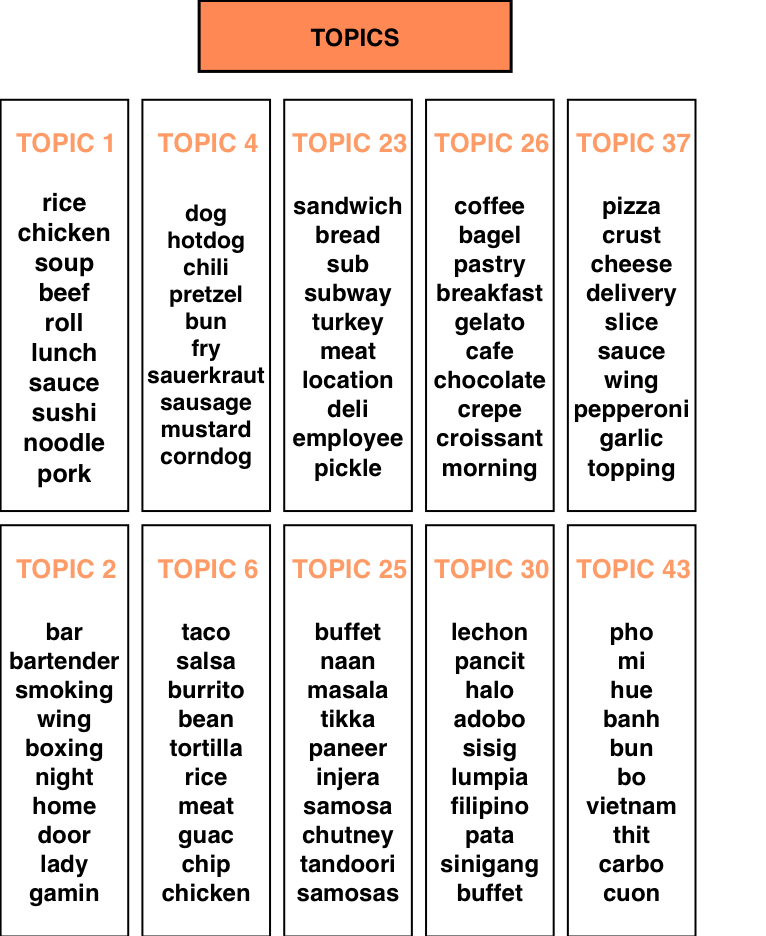
\includegraphics[width=1\linewidth]{topics.png}
\caption{Topics extracted from the Las Vegas reviews using OVI}
\end{figure} 

\noindent We obtained similar results using the NMF approach. The topics themselves were not our primary interested. As mentioned in the introduction, we were using these methods primarly for dimensional reduction purposes. We now present two different approaches to answer the question of classification using supervised and unsupervised machine learning.\\

%------------------------------------------------
\section{Supervised Classification}

\section{Unsupervised Clustering}
\subsection{Approach}

For this part of the project, we use the same features as for the supervised classification approach, i.e. the topic assignments. We wanted to see if it was possible to retrieve the original classification only based on the reviews. To do so and in order to check if our classification attempt was successful, we sampled about 1000 restaurants having tags in the following list of 6 categories: Sushi, Steakhouse, Seafood, Mexican, Sports and Breakfast \& Brunch. We then applied applied the following methodology.\\

Each restaurant is now represented as probability distribution over the latent topics. Using the Shannon distance (symmetric Kullback-Liebler Divergence), we created a distance matrix gathering information on how close 2 restaurants are based on their reviews. After many experimentations, we chose to transform this distance matrix into a weighted adjacency matrix:\\

\begin{compactitem}
\item $w_{ij} = 5$ if $d_{Shannon}(r_i,r_j)<1$,
\item $w_{ij} = 0.1$ otherwise.\\
\end{compactitem}

\noindent The choice of having a non-zero weight between two restaurants even though they are not "close" is motivated by the fact that many graph clustering algorithm and in particular the WalkTrap algorithm that we used and present next, will only work on a connected graph.\\

\noindent We then transformed this adjacency matrix in an unweighted graph and applied the Walktrap algorithm for community detection.\\

\subsection{The WalkTrap Algorithm}
The WalkTrap Algorithm is a community detection algorithm created by Pascal Pons and Matthieu Latapy \cite{Gr}. The algortihm runs in time $O(n^2\log n)$ and space $O(n^2)$ where $n$ is the number of vertices in the graph. As mentioned in their paper, "the intuition behind the Walktrap is that random walks on a graph tend to get trapped into densely connected parts corresponding to communities".\cite{Gr} It relies on a new metric used to evaluate the distance between two vertices in a graph:
 $$r_{ij} = \sqrt{\sum\limits_{k=1}^{n}\frac{(P^t_{ik}-P^t_{kj})^2}{d(k)}}$$
 where $P^t_{ik}$ is the transition probability in $t$ steps and $d(k)$ is the degree of node k (number of edges incident to the vertex). We can then generalise this distance between two vertices to a distance between two communities. Using this distance, we can now apply a hierarchical clustering algorithm.

\begin{algorithm}[H]
\caption{Walktrap Algorithm}\label{euclid}
\begin{algorithmic}[1]
\State Start with a partition $\mathcal{P}_1=\{\{v\}, v \in V\}$
\State Compute the distances between all adjacent vertices
\While {$\mathcal{P}_t\neq V$}
\State Merge 2 communities $\mathcal{C}_i$ and $\mathcal{C}_j$ in $\mathcal{P}_k$ and create a new partition $\mathcal{P}_{k+1}$
\State Evaluate the distances between the communities in this new partition
\EndWhile
\end{algorithmic}
\end{algorithm}

\noindent The choice of communities to merge in step 4 is made using Ward's method. We look at minimising the mean within-cluster variance:
$$\frac{1}{n_\mathcal{C}}\sum\limits_{\mathcal{C}\in\mathcal{P}_{k}}\sum\limits_{i\in\mathcal{C}}r^2_{i\mathcal{C}},$$
\noindent where $n_\mathcal{C}$ is the number of communities at iteration $k$, and $r_{i\mathcal{C}}$ is the distance from vertex i to its community $\mathcal{C}$.\\

\subsection{Results}

Running the algorithm from the \emph{igraph} in R, we outputted a dendogram (cf. Figure 3) representing the obtained clustering. We colored the tag of each business for a better readability.  It is not yet entirely clear to us how to get the optimum number of clusters. We were puzzled to see that the Walktrap algorithm indicated that a cut into 3 big clusters represented the optimum partition. Knowing the structure of the sampled restaurants, we decided to further investigate the dendogram. As one can see on Figure 3, cutting the tree at different heights, we can obtain 5 clear colored communities, corresponding to 5 of the 6 tags we pre-selected.\\

\noindent We summarized this classification using a confusion matrix: 
\begin{figure}[H]
\centering
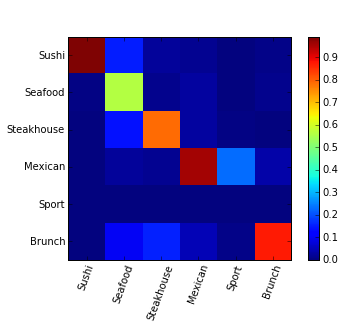
\includegraphics[width=1\linewidth]{confusion}
\caption{Confusion Matrix using the Walktrap Algorithm}
\end{figure}

\noindent With this method, we managed to detect 4 communities with great accuracy (over 80\%). Nevertheless, this classification still has some flaws and the most obvious one is the misclassification or even non-classification of the Sports bars (yellow). We focused a bit more on these venues and explored manually the tags associated with them. We noticed that these Sports bar were most of the time having other tags such as "Restaurants","Bar", "American" and some even "Mexican". Reviews for these venues might have been misallocated due to the proximity of types of food, drinks or "ambiance" with Mexican restaurants. It is nonetheless interesting to note that were grouped almost all together inside the Mexican restaurants, and that if we cut the three at the sixth level then they would all be gathered in 2 cliques.\\

\noindent It seems that this method will succeed in making a difference between communities of restaurants if they are almost exlusive. It seems very unlikely to discover a restaurant that one can identify as both a Mexican and a Sushi place or even a Sushi place specialising in Breakfast (unless its speciality is the takagoyaki, a type of Japanese omelette made by "rolling together several layers of cooked egg"). It was often the case that misclassified restaurant had the tag "Buffet" which is for our purpose of classification our worst ennemy as it will phagocytose many categories at once.

\begin{figure*}
\centering

\includegraphics[angle=90,width=0.25\linewidth]{den_ovi2-1.png}
\caption{Dendogram outputted by the Walktrap Algorithm}
\end{figure*}
\newpage

\section{Next steps}
Futur work could focus on the sub-cliques and try to get a finer classification by combining them with other features like check-ins, parking availability, etc. As a variant, we could also try a supervised LDA, where we use the existing categories as a response variable associated with each document and infer the joint model of the documents and the responses.

\section{conclusion}
By using a combination of unsupervised learning and graph theory, we managed to retrieve most of the original classification that is up to now still done by hand ! This work could result in an automation tool for Yelp to label properly its database. 

%----------------------------------------------------------------------------------------
%	REFERENCE LIST
%----------------------------------------------------------------------------------------

\nocite{*} % Insert publications even if they are not cited in the poster
\bibliographystyle{unsrt}
\bibliography{sample}
\end{multicols}


\end{document}



%----------------------------------------------------------------------------------------



